\section{Models and entailment in propositional logic}

\subsection{Validity and Soundness}

\begin{enumerate}[label=\alph*)]
    \item \textit{Generate the vocabulary of the following argument.}
    \item \textit{Translate the argument into propositional logic statements.}
    \item \textit{Add a premise (P4) to make the conclusion of the argument valid.} 
\end{enumerate}

\textit{P1 to P3 are the premises, C is the conclusion: }

\begin{itemize}
    \item \textit{(P1) If Peter’s argument is valid and all the premises of Peter’s argument are true, then Peter’s
    argument is sound.}
    \item \textit{(P2) If the premises of Peter’s argument entail the conclusion of Peter’s argument, then Peter’s
    argument is valid.}
    \item \textit{(P3) The premises of Peter’s argument entail the conclusion of Peter’s argument.}
    \item \textit{(C) Peter’s argument is sound.}
\end{itemize}

a) Vocabulary: 

\begin{itemize}
    \item $V$: Peter's argument is valid
    \item $P$: The premises of Peter's argument
    \item $S$: Peter's argument is sound
    \item $C$: The conclusion of Peter's argument
\end{itemize}

b) 

\begin{itemize}
    \item (P1): $V \land P \Longrightarrow S$
    \item (P2): $P \models C \Longrightarrow V$
    \item (P3): $P \models C$
    \item (C): $S$
\end{itemize}

c) 

To make the conclusion of the argument valid, one can add the premise: 

(P4): The Premises of Peter's argument are true. 

\subsection{Modelling}

\textit{For each of the following statements, determine if they are satisfiable by building the complete model
(truth table) and mark tautologies.}

I have given steps in the truth tables alternative lettering to save space in the tables. 

\begin{enumerate}[label=\alph*)]
    \item $ (p \Longleftrightarrow q) \Longrightarrow ((p \Longrightarrow r) \Longrightarrow (q \Longrightarrow r)) $ 
    
        \[
            \begin{array}{cccccccc}  
                \hline
                p & q & r & (p \Longleftrightarrow q) & (p \Longrightarrow r) & (q \Longrightarrow r) & (b \Longrightarrow c) & a \Longrightarrow (b \Longrightarrow c) \\
                & & & a & b & c & & \\
                \hline
                1 & 1 & 1 & 1 & 1 & 1 & 1 & 1 \\
                1 & 1 & 0 & 1 & 0 & 0 & 1 & 1 \\
                1 & 0 & 0 & 0 & 0 & 1 & 1 & 1 \\
                1 & 0 & 1 & 0 & 1 & 1 & 1 & 1 \\
                0 & 1 & 0 & 0 & 1 & 0 & 0 & 1 \\
                0 & 1 & 1 & 0 & 1 & 1 & 1 & 1 \\
                0 & 0 & 1 & 1 & 1 & 1 & 1 & 1 \\
                0 & 0 & 0 & 1 & 1 & 1 & 1 & 1 \\
            \end{array}
        \]
        

        As we can see this is a tautology as the expression is always true and thus it is also satisfiable. 
    \item $ (p \lor (\neg q \Longrightarrow r)) \Longrightarrow (q \lor (\neg p \Longrightarrow r)) $
    
        \[
            \begin{array}{cccccccc}  
                \hline
                p & q & r & (\neg q \Longrightarrow r) & (\neg p \Longrightarrow r) & (p \lor a) & (q \lor b) & (p \lor a) \Longrightarrow (q \lor b) \\
                & & & a & b & & & \\
                \hline
                1 & 1 & 1 & 1 & 1 & 1 & 1 & 1 \\
                1 & 1 & 0 & 1 & 1 & 1 & 1 & 1 \\
                1 & 0 & 0 & 0 & 1 & 1 & 1 & 1 \\
                1 & 0 & 1 & 1 & 1 & 1 & 1 & 1 \\
                0 & 1 & 0 & 1 & 0 & 1 & 0 & 0 \\
                0 & 1 & 1 & 1 & 1 & 1 & 1 & 1 \\
                0 & 0 & 1 & 1 & 1 & 1 & 1 & 1 \\
                0 & 0 & 0 & 0 & 0 & 0 & 0 & 1 \\
            \end{array}
        \]

        The statement is satisfiable. 
    \item $ (\neg (p \land (q \Longrightarrow \neg r))) \Longrightarrow ((p \Longrightarrow q) \land (p \Longrightarrow r)) $
    
        \[
            \begin{array}{ccccccccc}  
                \hline
                p & q & r & (q \Longrightarrow \neg r) & (p \Longrightarrow q) & (p \Longrightarrow r) & (p \land a) & (b \land c) & (\neg (p \land a)) \Longrightarrow (b \land c) \\
                & & & a & b & c & & & \\
                \hline
                1 & 1 & 1 & 0 & 1 & 1 & 0 & 1 & 1\\
                1 & 1 & 0 & 1 & 1 & 0 & 1 & 0 & 1\\
                1 & 0 & 0 & 1 & 0 & 0 & 1 & 1 & 1\\
                1 & 0 & 1 & 0 & 0 & 1 & 0 & 0 & 0\\
                0 & 1 & 0 & 1 & 1 & 1 & 0 & 1 & 1\\
                0 & 1 & 1 & 1 & 1 & 1 & 0 & 1 & 1\\
                0 & 0 & 1 & 1 & 1 & 1 & 0 & 1 & 1\\
                0 & 0 & 0 & 0 & 1 & 1 & 1 & 1 & 1\\
            \end{array}
        \]

        The statement is satisfiable. 
    \item $ (\neg (\neg p \Longrightarrow (q \land r))) \Longrightarrow (\neg (p \lor q) \land r) $ 
    
        \[
            \begin{array}{ccccccccc}  
                \hline
                p & q & r & (q \land r) & (p \lor q) & (\neg p \Longrightarrow a) & ( \neg b \land r) & (\neg c \Longrightarrow d) \\
                & & & a & b & c & d &  \\
                \hline
                1 & 1 & 1 & 1 & 1 & 1 & 1 & 1 \\
                1 & 1 & 0 & 0 & 1 & 1 & 1 & 1 \\
                1 & 0 & 0 & 1 & 1 & 1 & 1 & 1 \\
                1 & 0 & 1 & 0 & 1 & 1 & 1 & 1 \\
                0 & 1 & 0 & 0 & 1 & 0 & 1 & 1 \\
                0 & 1 & 1 & 1 & 1 & 1 & 1 & 1 \\
                0 & 0 & 1 & 0 & 0 & 0 & 1 & 1 \\
                0 & 0 & 0 & 1 & 0 & 1 & 0 & 1 \\
            \end{array}
        \]

        The statement is a tautology and is thus also satisfiable. 
\end{enumerate}

\subsection{Modelling 2}
\textit{Let $\phi$ be a sentence that contains three atomic constituents and let the truth conditions of $\phi$ be defined
by the truth table below. Write a propositional logic statement that contains $p$, $q$, and $r$ as constituents,
and that is equivalent to $\phi$.}

\[
\begin{array}{cccc}
    \hline 
    p & q & r & \phi \\
    \hline 
    1 & 1 & 1 & 1 \\
    1 & 1 & 0 & 1 \\
    1 & 0 & 1 & 0 \\
    1 & 0 & 0 & 1 \\
    0 & 1 & 1 & 1 \\
    0 & 1 & 0 & 1 \\
    0 & 0 & 1 & 0 \\
    0 & 0 & 0 & 1 \\
    \hline
\end{array}
\]

A statement that contains $p$, $q$, and $r$ and is equivalent to $\phi$ is

$$ ((p \Longrightarrow r) \Longrightarrow (p \Longrightarrow q)) \land ((r \Longrightarrow p) \lor q) $$



\section{Resolution in propositional logic}

\subsection{Conjuctive Normal Form}
\textit{Convert each of the following sentences to their Conjuctive Normal Form (CNF).}

\begin{enumerate}[label=\alph*)]
    \item $ p \Longleftrightarrow q $ 

        \begin{align*}
            &\Rightarrow (p \Longrightarrow q) \land (q \Longrightarrow p) \\
            &\Rightarrow (\neg p \lor q) \land (\neg q \lor p) \\
        \end{align*}

    \item $ \neg ((p \Longrightarrow q) \land r ) $
    
        \begin{align*}
            &\Rightarrow \neg ((\neg p \lor q) \land r) \\
            &\Rightarrow (p \land \neg q) \lor (\neg r) \\
            &\Rightarrow (p \lor \neg r) \land (\neg q \lor \neg r)  \\
        \end{align*}

    \item $ ((p \lor q) \lor (r \land (\neg (q \Longrightarrow r)))) $
    
        \begin{align*}
            &\Rightarrow (p \lor q \lor (r \land (\neg (\neg q \lor r)))) \\
            &\Rightarrow (p \lor q \lor (r \land (q \land \neg r))) \\
            &\Rightarrow (p \lor (r \land q \land \neg r)) \land (q \lor (r \land q \land \neg r)) \\
            &\Rightarrow (p \lor r) \land (p \lor q) \land (p \lor \neg r) \land (q \lor r) \land ( \lor p) \land (q \lor \neg r) \\
            &\Rightarrow (p \lor q \lor r) \land (p \lor q \lor \neg r) \\
            &\Rightarrow (p \lor q)
        \end{align*}

    \item \textit{Is the solution to c) really a CNF?} 
    
        As the solution to c) can be simplified to $(p \lor q)$ the solution is not a true CNF, but rather a disjunction of literals. It can still be written as a CNF with $r$ and $\neg r$, but it is in practice $(p \lor q)$. 

\end{enumerate}

\subsection{Inference in propositional logic}
\textit{Use resolution to conclude $r$ from the following statements.}

\begin{enumerate}[label=\alph*)]
    \item $ (p \Longrightarrow q) \Longrightarrow q $
    
        \begin{align*}
            & (\neg p \lor q) \Longrightarrow q \\
            & \neg (\neg p \lor q) \lor q \\
            & p \land \neg q \lor q \\
            & p 
        \end{align*}

    \item $ p \Longrightarrow r $ 
    
        \begin{align*}
            \neg p \lor r
        \end{align*}

    \item $ (r \Longrightarrow s) \Longrightarrow (\neg (s \Longrightarrow q)) $

        \begin{align*}
            & (\neg r \lor s) \Longrightarrow (\neg (\neg s \lor q)) \\
            & \neg (\neg r \land s) \lor ( s \land \neg q) \\
            & r \land (s \land \neg q)
        \end{align*}

        We can see that from a) and b) we get the clauses $p$ and $(\neg p \lor r)$ from these two we can infer r. Thus r can be concluded from the statements.
        
        $$\frac{p, \hspace{0.3cm} \neg p \lor r}{r}$$

\end{enumerate}

\newpage

\section{Representation in First-Order Logic (FOL)} 

\textit{Consider the following baseball vocabulary:}

\begin{enumerate}
    \item \textit{Pitcher(p)} is a predicate where person $p$ is a pitcher.
    \item \textit{flies($ p_1, p_2 $)} is a predicative where person $p_1$ flies out to person $p_2$.
    \item \textit{Centerfielder(p)} is a predicate where person $p$ is a centerfielder.
    \item \textit{scores(p)} is a predicate where person $p$ scores.
    \item \textit{friend($p_1, p_2$)} is a predicate where person $p_1$ is the friend of person $p_2$ (but not vice versa).
    \item \textit{Robinson, Crabb, Samson, Jones} are constants denoting persons.
\end{enumerate}

\textit{Now look at the following translations of natural language into first order logic statements describing
a baseball game. \textbf{Using the provided vocabulary, translate the conclusion of each of the
following arguments into an FOL statement.}}

\begin{enumerate}[label=\alph*)]
    \item \textbf{Argument A} 
    
        \textit{Only pitchers fly out to Robinson. Crabb scores only if Samson flies out to Robinson and Robinson is a
        centerfielder. Crabb scores.}

        Conclusion: \textit{Samson is a pitcher.}

        \begin{itemize}
            \item $\forall x: \left[ flies(x,\, Robinson) \Longrightarrow Pitcher(x) \right]$
            \item $scores(Crabb) \Longrightarrow (flies(Samson,\, Robinson) \land Centerfielder(Robinson))$
            \item $scores(Crabb)$
        \end{itemize}
        \vspace{0.5cm}

        \textbf{Conclusion as FOL statement:} $Pitcher(Samson)$

        \vspace{0.5cm}

    \item \textbf{Argument B}
    
        \textit{No centerfielder who does not score has any friends. Robinson and Jones are both centerfielders. Any
        centerfielder who flies out to Jones does not score. Robinson flies out to Jones.}

        Conclusion: \textit{Jones is not a friend of Robinson}

        \begin{itemize}
            \item $\forall x: \left[ (Centerfielder(x) \land \neg scores(x)) \Longrightarrow \neg \exists y: \left[friend(y,\,x)\right] \right]$
            \item $Centerfielder(Robinson) \land Centerfielder(Jones)$
            \item $\forall x: \left[ (Centerfielder(x) \land flies(x,\, Jones)) \Longrightarrow \neg scores(x) \right]$
            \item $flies(Robinson,\,Jones)$
        \end{itemize}

        \vspace{0.5cm}

        \textbf{Conclusion as FOL statement:} $\neg friend(Jones, Robinson)$

        \vspace{0.5cm}

\end{enumerate}

\newpage

\section{Resolution in FOL}

\textit{Using resolution, prove the conclusions from \textbf{Arguments A} and \textbf{B} from exercise 3}

\textbf{Argument A} 

First, we need to write the clauses of the arguments on CNF: 

\begin{itemize}
    \item $\forall x: \left[ flies(x,\, Robinson) \Longrightarrow Pitcher(x) \right]$

    \begin{align*}
        & \forall x: \left[ \neg flies(x,\, Robinson) \lor Pitcher(x) \right] \\
        & \neg flies(x,\, Robinson) \lor Pitcher(x)
    \end{align*}

    \item $scores(Crabb) \Longrightarrow (flies(Samson,\, Robinson) \land Centerfielder(Robinson))$
    
    \begin{align*}
        & \neg scores(Crabb) \lor (flies(Samson,\, Robinson) \land Centerfielder(Robinson)) \\
        & (\neg scores(Crabb) \lor flies(Samson,\, Robinson)) \land (\neg scores(Crabb) \lor Centerfielder(Robinson)) 
    \end{align*}

    \item $scores(Crabb)$
    \item $Pitcher(Samson)$
\end{itemize}

Thus we get the clauses: 

\begin{enumerate}
    \item[1.1] $\neg flies(x,\, Robinson) \lor Pitcher(x)$
    \item[1.2] $\neg scores(Crabb) \lor flies(Samson,\, Robinson)$
    \item[2] $\neg scores(Crabb) \lor Centerfielder(Robinson)$
    \item[3] $scores(Crabb)$
    \item[$\neg$G] $\neg Pitcher(Samson)$
\end{enumerate}

which by resolution yields

\begin{figure}[!h]
    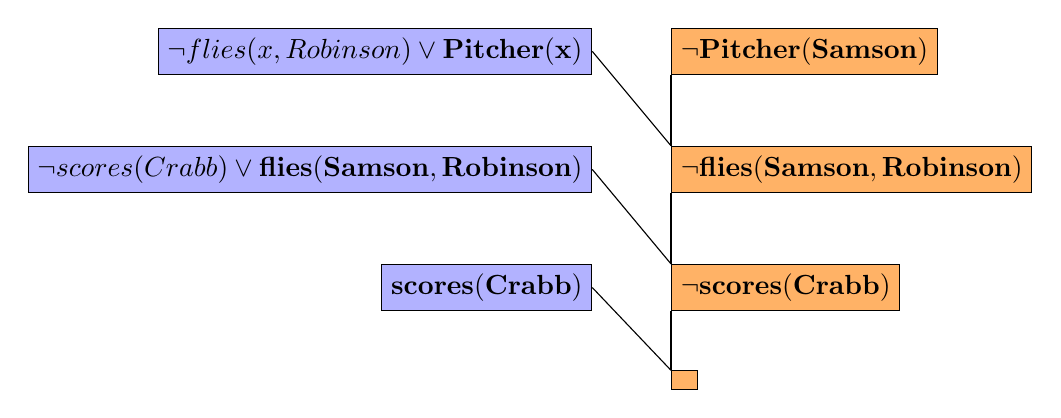
\begin{tikzpicture}
        \node[rectangle, draw, anchor=south east, fill=blue!30] (a) at (0,0) {$\neg flies(x, Robinson) \lor \mathbf{Pitcher(x)}$};
        \node[rectangle, draw, anchor=south west, fill=orange!60] (b) at (1,0) {$\mathbf{\neg Pitcher(Samson)}$};
        \node[rectangle, draw, anchor=south west, fill=orange!60] (c) at (1,-1.5) {$\mathbf{\neg flies(Samson, Robinson)}$};
        \node[rectangle, draw, anchor=south east, fill=blue!30] (d) at (0,-1.5) {$\neg scores(Crabb) \lor \mathbf{flies(Samson, Robinson)}$};
        \node[rectangle, draw, anchor=south east, fill=blue!30] (e) at (0,-3) {$\mathbf{scores(Crabb)}$};
        \node[rectangle, draw, anchor=south west, fill=orange!60] (f) at (1,-3) {$\mathbf{\neg scores(Crabb)}$};
        \node[rectangle, draw, anchor=south west, fill=orange!60] (g) at (1,-4) {$\;$};

        \draw (a.east) -- (c.north west);
        \draw (b.south west) -- (c.north west);
        \draw (d.east) -- (f.north west);
        \draw (c.south west) -- (f.north west);
        \draw (e.east) -- (g.north west);
        \draw (f.south west) -- (g.north west);
        
    \end{tikzpicture}
\end{figure}

as $\neg Pitcher(Samson)$ is unsatisfiable by resolution the conclusion is proven. 

\newpage

\textbf{Argument B}

\begin{itemize}
    \item $\forall x: \left[ (Centerfielder(x) \land \neg scores(x)) \Longrightarrow \neg \exists y: \left[friend(y,\,x)\right] \right]$
        \begin{align*}
            & \forall x: \left[ \neg (Centerfielder(x) \land \neg scores(x)) \lor \forall y: \left[\neg friend(y,\,x)\right] \right] \\
            & (\neg Centerfielder(x) \land scores(x)) \lor \neg friend(F(x),\,x) \\
            & (\neg Centerfielder(x) \lor \neg friend(F(x),\,x)) \land (scores(x) \lor \neg friend(F(x),\,x)) 
        \end{align*}

    \item $Centerfielder(Robinson) \land Centerfielder(Jones)$
    \item $\forall x: \left[ (Centerfielder(x) \land flies(x,\, Jones)) \Longrightarrow \neg scores(x) \right]$
        \begin{align*}
            & \forall x: \left[ \neg (Centerfielder(x) \land flies(x,\, Jones)) \lor \neg scores(x) \right] \\
            & (\neg Centerfielder(x) \land \neg flies(x,\, Jones)) \lor \neg scores(x) \\
            & (\neg Centerfielder(x) \lor \neg scores(x)) \land (\neg flies(x,\, Jones) \lor \neg scores(x))
        \end{align*}

    \item $flies(Robinson,\,Jones)$
    \item $\neg friend(Jones, Robinson)$
\end{itemize}

The clauses are then: 

\begin{enumerate}
    \item[1.1] $ \neg Centerfielder(x) \lor \neg frien d(F(x),\,x) $
    \item[1.2] $ scores(x) \lor \neg friend(F(x),\,x) $
    \item[2.1] $ Centerfielder(Robinson) $
    \item[2.2] $ Centerfielder(Jones) $
    \item[3.1] $ \neg Centerfielder(x) \lor \neg scores(x) $
    \item[3.2] $ \neg flies(x,\, Jones) \lor \neg scores(x) $
    \item[4] $ flies(Robinson,\,Jones) $
    \item[$\neg$G] $ friend(Jones, Robinson) $
\end{enumerate}

which yields: 


\begin{figure}[!h]
    \begin{center}
    \makebox[\textwidth]{
    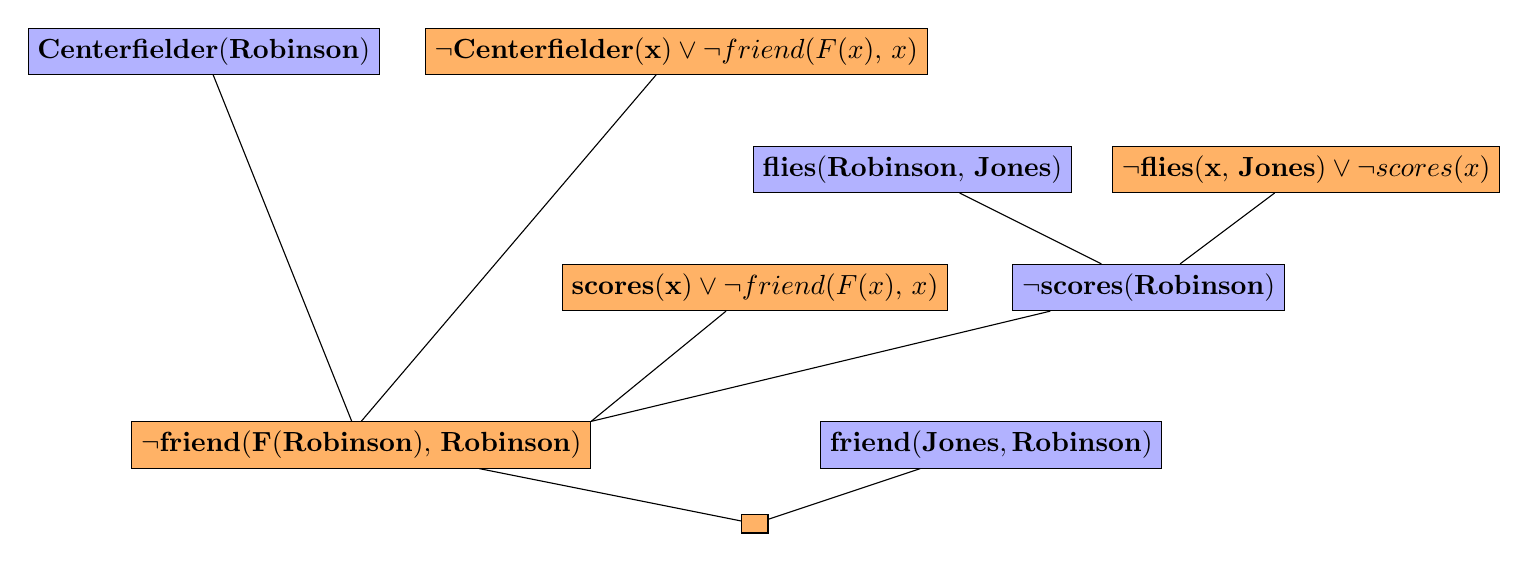
\begin{tikzpicture}
        \node[rectangle, draw, fill=blue!30] (a) at (-2,0) {$\mathbf{Centerfielder(Robinson)}$};
        \node[rectangle, draw, fill=orange!60] (b) at (4,0) {$\mathbf{\neg Centerfielder(x)} \lor \neg friend(F(x),\,x)$};
        \node[rectangle, draw, fill=orange!60] (c) at (0,-5) {$\mathbf{\neg friend(F(Robinson),\,Robinson)}$};
        \node[rectangle, draw, fill=blue!30] (d) at (7,-1.5) {$\mathbf{flies(Robinson,\,Jones)}$};
        \node[rectangle, draw, fill=orange!60] (e) at (12,-1.5) {$\mathbf{\neg flies(x,\, Jones)} \lor \neg scores(x)$};
        \node[rectangle, draw, fill=blue!30] (f) at (10,-3) {$\mathbf{\neg scores(Robinson)}$};
        \node[rectangle, draw, fill=orange!60] (g) at (5,-3) {$\mathbf{scores(x)} \lor \neg friend(F(x),\,x) $};
        \node[rectangle, draw, fill=blue!30] (h) at (8,-5) {$\mathbf{friend(Jones, Robinson)} $};
        \node[rectangle, draw, fill=orange!60] (i) at (5,-6) {$\;$};

        \draw (a) -- (c);
        \draw (b) -- (c.north);
        \draw (d) -- (f);
        \draw (e) -- (f);
        \draw (f) -- (c.north east);
        \draw (g) -- (c.north east);
        \draw (c) -- (i);
        \draw (h) -- (i);
    \end{tikzpicture}}
    \end{center}
\end{figure}

given $F(Robinson) = Jones$, $friend(Jones, Robinson)$ is unsatisfiable by resolution and the conclusion is proven. 